%\documentclass[times, 10pt, twocolumn]{article}
%\documentclass[conference,final]{IEEEtran}

\documentclass{rspublic}

%------------------------------------------------------------------------- take
%the % away on next line to produce the final camera-ready version
%\pagestyle{empty}

\usepackage{graphicx}
\usepackage{float}
\usepackage{times}
\usepackage{multirow}
\usepackage{listings}
\usepackage{paralist}
\usepackage{wrapfig}
\usepackage[small,it]{caption}
%%\usepackage{multirow}
\usepackage{ifpdf}
\usepackage{subfigure}
\usepackage{url}

%%\usepackage{subfig}
%\usepackage[pdftex]{graphicx}
%\usepackage{harvard}
%\usepackage{pdfsync}

%Bibliography
\usepackage{natbib}
\usepackage{listings}
\usepackage{keyval}
\usepackage{color}
\definecolor{listinggray}{gray}{0.95}
\definecolor{darkgray}{gray}{0.7}
\definecolor{commentgreen}{rgb}{0, 0.4, 0}
\definecolor{darkblue}{rgb}{0, 0, 0.4}
\definecolor{middleblue}{rgb}{0, 0, 0.7}
\definecolor{darkred}{rgb}{0.4, 0, 0}
\definecolor{brown}{rgb}{0.5, 0.5, 0}
\definecolor{orange}{rgb}{1,0.5,0}

\lstdefinestyle{myListing}{ frame=single, backgroundcolor=\color{listinggray},
  %float=t,
  language=C, basicstyle=\ttfamily \footnotesize, breakautoindent=true,
breaklines=true tabsize=2, captionpos=b, aboveskip=0em,
  %numbers=left, numberstyle=\tiny
}

\lstdefinestyle{myPythonListing}{ frame=single,
backgroundcolor=\color{listinggray},
  %float=t,
  language=Python, basicstyle=\ttfamily \footnotesize,
breakautoindent=true, breaklines=true tabsize=2, captionpos=b,
  %numbers=left, numberstyle=\tiny
}

\title[Understanding Performance Implications of Distributing Data for
Data-Intensive Applications]{Understanding Performance Implications of
Distributing Data for Data-Intensive Applications}


\author[Miceli, Miceli, Rodriguez-Milla, Jha]{ Christopher Miceli$^{1}$,
Michael Miceli$^{1}$, Bety Rodriguez-Milla$^{1}$, Shantenu Jha$^{1,2,*}$ \\
\small{\emph{$^{1}$Center for Computation \& Technology, Louisiana State
University, USA}} \\  \small{\emph{$^{2}$Department of Computer Science,
Louisiana State University, USA}} \\ {\footnotesize {\hspace{0.0 in}
$^*$Corresponding Author sjha@cct.lsu.edu}} }

%\date{}

\def\acknowledgementname{Acknowledgements} \newenvironment{acknowledgement} 

% {\section*{\acknowledgementname}%\parindent=0pt% }

\newif\ifdraft \drafttrue \ifdraft \newcommand{\fixme}[1]{ { \bf{ ***FIXME: #1
}} } \newcommand{\jhanote}[1]{ {\textcolor{red} { ***Jha: #1 }}}
\newcommand{\micnote}[1]{ {\textcolor{blue} { ***Michael: #1 }}} 
\newcommand{\betynote}[1]{ {\textcolor{orange} { ***Bety: #1 }}}
\else
\newcommand{\jhanote}[1]{} \newcommand{\micnote}[1]{}\newcommand{\betynote}[1]{} \newcommand{\fixme}[1]{}
\fi

\begin{document} \maketitle

\micnote{This can't be more than 200 words. The summary should be
concise and informative. It should be complete by itself, and must not
contain references or unexplained abbreviations. It should not only
indicate the general scope of the article but also state the main
results and conclusions. Please note that footnotes are not used.}

\begin{abstract}{data-intensive computing, distributed computing,
    cloud computing, grid computing} 
Grids, clouds and cloud-like infrastructures are capable of supporting
problems that are data-intensive. There are interesting and unique
performance issues that appear as the volume of data increases which
require scalable data placement and management techniques, as well as
novel approaches to the relative placement of data and computational
workload.  This paper aims to understand the factors that
determine the performance of a representative data-intensive
application, and to understand the performance trade-off in design
decisions. This is analogous to benchmarking the performance of an
application on a new platform. We analyse two techniques to manage data
placement. One focuses on data placement and the other on worker
placement. The goal of this paper is to understand techniques for
distributing data in a distributed environment and understand
performance issues associated with these techniques.
\end{abstract}

% Grids, clouds and cloud-like
%   infrastructures are capable of supporting problems that are
%   data-intensive. There are interesting and unique performance issues
%   that appear as the volume of data increases which require scalable
%   data placement and management techniques, as well as novel
%   approaches to the relative placement of data and computational
%   workload.  The aim of this paper is to understand the factors that
%   determine the performance of a representative data-intensive
%   application, and to understand the performance trade-off in design
%   decisions. This is analagous to benchmarking the performance of an
%   application on a new platform. We analyse two techniques to manage
%   data placement. One focuses on data placement and the other on
%   worker placement. The goal of this paper is to understand techniques
%   for distributing data in a distributed environment and understand
%   performance issues associated with these techniques.

\section{Introduction} Data-intensive computing is a fast growing area
of computer science. A good example of this is Google, which processes
around 20 petabytes of data per day ~\citep{google}, and trends show
continuing growth. It has become very important that a distributed
application developer takes precautions when placing, scheduling, and
managing large volumes of data. Careless placement can adversely affect
system performance greatly. It is decisive then to determine whether to
move input data to the computational resource, or the computational
workload to the input data. There are two ways to handle this issue,
with distributed filesystems, which focus on data placement, or with the
use of an intelligent framework, which focuses on worker placement. 

\jhanote{refine} Different metrics of concern for parallel
vs. distributed data (I/O).  I/O typically dominated by Bandwidth for
Cluster/Parallel systems, I/O dominated by latency. The challenge in
load balancing for the former is often disc or bus-limited at the
hardware level, while at the software/application level the challenge
is to increase concurrent I/O with computation. For distributed
systems and applications the challenge is to find an optimal
distribution strategy, that takes into account the ratio of
computation workload to data distribution.  Data privacy, security and
access policy is a crucial non-technical issue for distributed
applications.  


Distributed filesystems (DFS), motivated in part by developments in
cloud computing, are useful and effective tools to consider for
data-intensive scientific applications. A DFS controls the data
placement and provides a uniform interface for accessing files on
multiple hosts. Frequently, there is more than one copy of the input
data for fault-tolerance reasons, consequently, the added issue of
deciding between the two or more replicas becomes relevant. While a DFS
removes the responsibility of replica management and data server
placement, the abstraction often increases the difficulty in determining
where in the DFS the data is being stored. This puts pressure on a
DFS's protocols and internal algorithms to perform well. Despite this,
the DFS replication may alleviate this issue by placing replicas in
locations where computational resources reside. A downfall of DFSs is
the inability to make the decision of whether to move the input data, or
the computational workload. It can only focus on minimizing poor data
management. The most common parameters in determining the performance of
using a DFS are the performance overhead compared to a normal local
filesystem, number of replicas of each datum/file, and the number of
servers. In our experiments, we use the stable open source distributed
filesystem CloudStore (formerly KFS), which is written in C++ released
under the Apache License Version 2.0. It is inspired by the highly
successful Google Filesystem, GFS ~\citep{cloudstore_web}, which is
closed source and unavailable for research. CloudStore was chosen for
its high performance focus, C++ implementation, and its source code
availability. It also provides a means to automatically replicate data
on different hosts to provide efficient data access and fault tolerance. 

Our intelligent framework method differs from a DFS in that it
determines where data is and where the work should go. 
Determining data location can be as simple as
looking at the IP address of the worker and seeing geographically where
it is located or as complicated as using network analyses tools to
determine the optimal data transfer minimization time. 
For this method, we use gridFTP, a tool that is used to transfer
files across machines in a grid. It is
specifically designed for high-bandwidth networks. GridFTP is provided by
the Globus Toolkit, an open source software toolkit
released under the Apache License version 2.0. Globus provides tools used
to create and manage grid infrastructures. 

In this paper, we provide some initial approaches to answer ``To
distribute or not to distribute data, is the question''. Our research
focuses on understanding the performance trade-offs of a DFS compared to
''regular'' distribution and placement techniques, as well as more
advanced intelligent distribution methods and finding how they handle
different data-sets and what there performance patterns are. This paper
also aims to determine how sensitive the performance is in the context
of a real data-intensive distributed applications.

\section {Methodology (change to a better title)} We use an application
based upon a grid-enabled All-Pairs abstraction in SAGA (Simple API for
Grid Applications, see Sec. \ref{Sec:SAGA}). This abstraction applies an
operation on two data-sets such that every possible pair containing one
element from the first set and one element from the second set has some
operation applied to it.~\citep{Interop, AllPairs} Essentially,
All-Pairs is a function of two sets, $A$ and $B$, with number of
elements $m$ and $n$, respectively, which creates a matrix $M$. Each
element $M_{i,j}$ is the result of the operation $f$ applied to the
elements $A_i$ and $B_j$.
\begin{eqnarray}
 AllPairs(A, B, f) & \rightarrow & M_{m \times n}, \\
\mbox{where} \quad M_{i,j} & = & f(A_{i},B_{j})
 \end{eqnarray}
 
The result of this application is stored in a matrix. The application
spawns distributed jobs to run sets of these function operations.
Examples of problems that fall into this category are image comparison
for facial recognition, and genome comparison. This paper uses genome
comparisons to find the best matching gene in a genome.
\begin{figure}[!ht]
 \begin{center}
     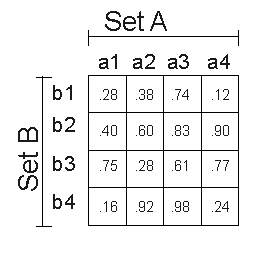
\includegraphics[width=0.40\textwidth]{data/allpairs-exp.pdf}
\end{center}
\caption{\small An example result from an All-Pairs enabled
application.  Every matrix element is the percentage equivalent to the
genomes on the axes.} \label{Fig:SAGA1}
\end{figure}

The problem becomes determining which pairs to put into a set and with
which distributed resource to run that set. If transferring data to the
job takes too long, we spend more time on data management than
computation.  There may be a resource capable of the work that may be
slower than others, but able to be accessed in a relatively quick manner
via the network, correcting for this lack of computational ability.
Therefore, we introduce the idea of network-closeness. A network-close
data-set takes a small amount of time to transfer to the work location.
A network-far data-set is just the opposite. A network-far data-set
takes a long time to transfer to the work location. If there is an
unprocessed data-set collocated or network-close with the job, then the
assignment of that worker to that data-set would have benefits. If there
is no unprocessed data-set that is network-close to the job, still we
assign data that may be network-far, in case the network-close job
failed or there is no available jobs network-close to the data-set.

%There are at least two types of data-intensive applications: the first
%where the actual data generated is large; the second type is where the
%data generated is small, but the volume of data on which computation
%occurs is very large. The application we used, has relatively small
%input and relatively small output, but the manner of processing causes
%many data reads. This type of application can be classified as having
%a large data throughput. \jhanote{Can you elaborate on different
%types of data-intensive applications? What kind is an ImageMagic
%based application?}

Our genome comparison application can be classified as having a large
data throughput, as, even though it has large input $O$(GB) and
relatively small output $O$(KB), the manner of processing causes many
data reads. SAGA~\citep{saga_url} allows our application to handle
seamlessly the DFS and gridFTP based data stores on clouds and grids.
This allows the same exact application to be used for all of our
experiments. 

\section{SAGA and SAGA-based Frameworks for Large-Scale and
  Distributed Computation}\label{Sec:SAGA}

%\alnote{removed the first paragraph - duplicated content}
% SAGA~\cite{saga_url} provides a simple, POSIX-inspired API to the most
% commonly required distributed functionality at a sufficiently
% high-level of abstraction so as to be independent of the divers\ e and
% dynamic Grid environments.

The Simple API for Grid Applications (SAGA) is an API
standardization effort within the Open Grid Forum
(OGF)~\cite{saga_gfd90}, an international standards development body
concerned primarily with standards for distributed computing. SAGA
provides a simple, POSIX-style API to the most common Grid functions
at a sufficiently high-level of abstraction so as to be independent of
the diverse and dynamic Grid environments. The SAGA specification
defines interfaces for the most common Grid-programming functions
grouped as a set of functional packages (Fig.~\ref{Fig:SAGA1}). Some
key packages are:

\begin{figure}[!ht]
 \begin{center}
     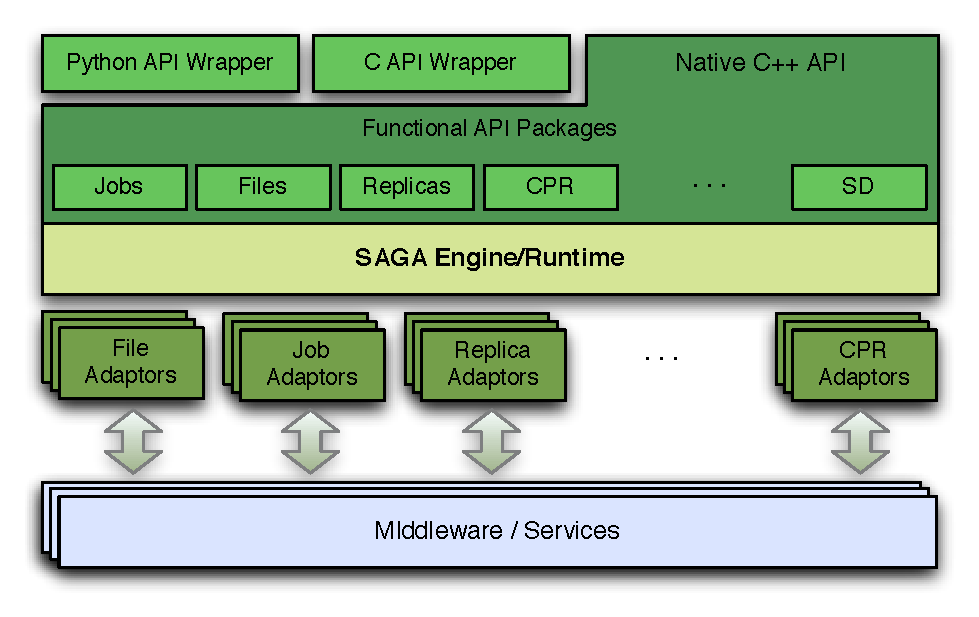
\includegraphics[width=0.40\textwidth]{stci_saga_figures-1.pdf}
    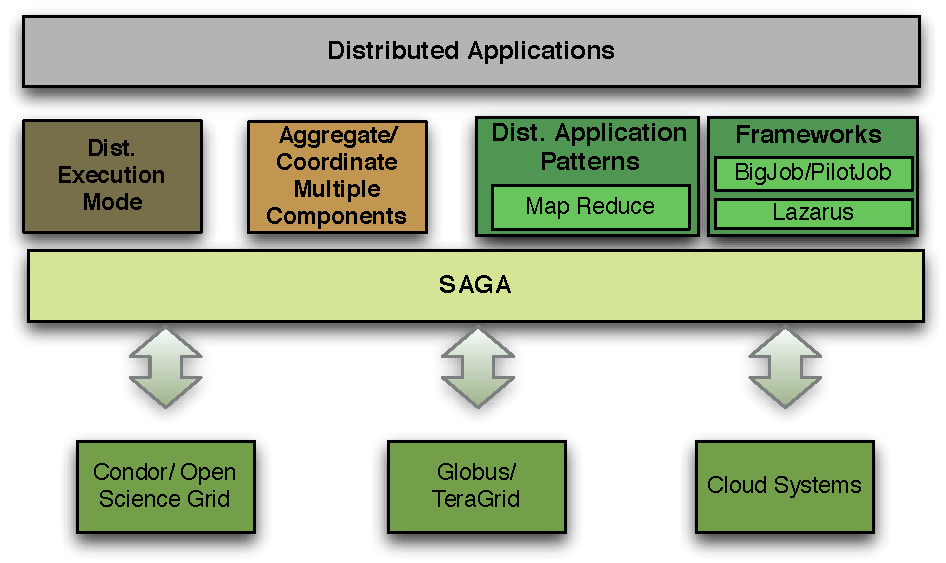
\includegraphics[width=0.45\textwidth]{distributed_applications_saga_figure.pdf}
\end{center}
\caption{\small [L] Layered schematic of the different components of
  the SAGA landscape. At the topmost level is the simple integrated
  API which provides the basic functionality for distributed
  computing. Our BigJob abstraction is built upon this SAGA layer
  using Python API bindings. [R] Showing the ways in which SAGA can be
  used to develop distributed applications.  The different shaded box
  represent the three different types; frameworks in turn can capture
  either common patterns or common application
  requirements/characteristics.} \label{Fig:SAGA1}
\end{figure}

\begin{itemize}
\item File package - provides methods for accessing local and remote
 filesystems, browsing directories, moving, copying, and deleting
 files, setting access permissions, as well as zero-copy reading and
 writing.
\item Job package - provides methods for describing, submitting,
 monitoring, and controlling local and remote jobs. Many parts of
 this package were derived from the largely adopted
 DRMAA % ~\cite{drmaa_url}                                                                                           
 specification.
\item Stream package - provides methods for authenticated local and
 remote socket connections with hooks to support authorization and
 encryption schemes.
\item Other Packages, such as the RPC (remote procedure call) and Replica
 package.
\end{itemize}

In the absence of a formal theoretical taxonomy of distributed
applications, Fig.~\ref{Fig:sagaapps} can act a guide.  Using this
classification system, there are three types of distributed
applications: (i) Applications where local functionality is swapped
for distributed functionality, or where distributed execution modes
are provided.  A simple but illustrative example is an ensemble of an
application that uses distributed resources for bulk submission. Here,
the application remains unchanged and even unaware of its distributed
execution, and the staging, coordination, and management are done by
external tools or agents. Most application in this category are
classified as implicitly distributed.  (ii) Applications that are
naturally decomposable or have multiple components are then aggregated
or coordinated by some unifying or explicit mechanism.  DAG-based
workflows are probably the most common example of applications in this
category.
% (ii) Applications that are developed using well known
% patterns, % for example MapReduce, which in turn is implemented using % infrastructure independent programming systems such as SAGA;
Finally, (iii) applications that are developed using frameworks, where
a framework is a generic name for a development tool that supports
specific application characteristics (e.g., hierarchical job
submission), and recurring patterns (e.g., MapReduce, data
parallelism) and system functionality.  SAGA has been used to develop
system-level tools and applications of each of these types.


% \begin{figure}[!ht]
%   \begin{center}
%     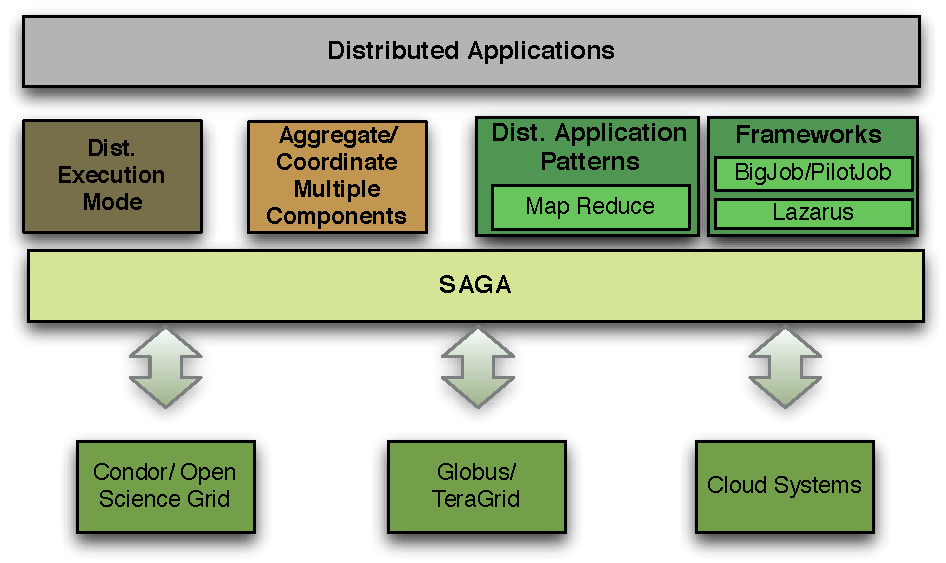
\includegraphics[width=0.45\textwidth]{distributed_applications_saga_figure.pdf}
%   \end{center}
%   \caption{\small Showing the ways in which SAGA can be used to
%     develop distributed applications.  The different shaded box
%     represent the three different types; frameworks in turn can
%     capture either common patterns or common application
%     requirements/characteristics. \label{Fig:sagaapps}}
% \end{figure}

It is important to note that SAGA provides the basic API to implement
distributed functionality required by applications (typically used
directly by the first category of applications), and is also used to
implement higher-level APIs, abstractions, and frameworks that, in
turn, support the development, deployment and execution of distributed
applications~\cite{saga_gmac09}. In Ref.~\cite{saga_montage_escience09} we
discussed how SAGA was used to implement a higher-level API to support
workflows. In this paper, we will discuss how SAGA can be used to
implement runtime frameworks to support the efficient execution of the
distributed applications.


\section{Performance Measurement and Analysis} We developed three types
of experiments in order to compare distributed filesystems with manual
file management. There are many questions we try to answer.  Does a
distributed filesystem grow more slowly than manual placement of data?
When manually handling data, what are the advantages of being able to
move work to data to the work? For this, we find the time to completion
$t_c$, which is a function of pre-processing time -- the dominant
component of which is the time for transfer -- $t_x$, I/O time
$t_{I/O}$, which is the time it takes to read and write files, and the
time to compute $t_{compute}$, which is the time it takes for genomes to
be compared, i.e.,
 \begin{equation}
t_c = t_x + t_{I/O} + t_{compute}.
\end{equation}
We focus on three variables to measure $t_c$: degree of distribution,
data dependency, and workload. Degree of distribution is defined as
the number of resources that are utilized for a given
computation/problem. For example, if data is distributed over 3
machines $D_d$ is 3; if data is distributed over three machines but
the computational tasks over 4 machines, the $D_d$ is 4.

\subsection{Experimental Configuration}

As explained before, for our experiments, we used an All-Pairs
implementation that utilises SAGA. An XML configuration file defines
various initial parameters which alter the behavior of our All-Pairs
implementation.  Such a file defines the location of the data that
comprises the two input sets, the grouping of pairs from these sets into
sets to be provided to the compute resources, and the available machines
that will perform the operation on these sets of pairs. The application
takes these sets of pairs and maps them to a computational resource
dynamically at run-time.  

Furthermore, variables external to the All-Pairs implementation also
influence experimental results. The following experiments can be
completely described by a tuple of the following form
 \begin{equation}
(c_s, N_c, M_c, fs, m,r),
\label{Eq:tuple}
\end{equation}
where $c_s$ is the total amount of data in each file of a set (i.e.,
$c_s=\mbox{\textit{chunk} size}$); $N_c$ is the number of work-loads
that the total work is decomposed into, i.e., number of work
assignments generated; $M_c$ is a comma separated list, of the machine 
configurations, of the
following form: $X(c, d)$ where $X$ is a shorthand reference for the
computational resource, $c$ shows if the computational resource $X$
was used in the computational workloads/calculations, and $d$ if the
computational resource $X$ assisted in data storage, both have a
yes/no $(Y/N)$ value.; $fs$ is the type of filesystem used; $m$ is the
method used to access that filesystem; and $r$ is the degree of
replication utilized in the experiment (with a default value of 1).
 However, for CloudStore, we investigate the performance with 
 $r = 1, 2 \mbox{ and } 3$.

In our experiments, we have three $(fs, m)$ configurations, and five $X$
configurations. Our $(fs, m)$ configurations are $(L,L)=(\mbox{local,
local})$, $(L,G)=(\mbox{local, gridFTP})$, and $(C,D)=(\mbox{CloudStore,
direct})$. By direct we mean, CloudStore is \jhanote{Finish this
setence!} Our $X$ configurations are enumerated in Table
\ref{Tab:Configs} below.  For one machine, $C1=X_1(Y,Y)$, where resource
$X_1$ has both the data and the computing; for two machines, we have
three configurations, and for three machines we only work with only one
configuration.

\begin{table}
\begin{center}
    \begin{tabular}{ | l | l |}
    \hline
    Configurations & $X(c,d)$; $c= \mbox{compute}$, $d=\mbox{data storage}$  \\ \hline
    $C1$ & $X_1(Y,Y)$  \\ \hline    
    $C2$ & $X_1(Y,N), X_2(N,Y)$ \\ \hline
    $C3$ & $X_1(Y,Y), X_2(N,Y)$ \\ \hline
    $C4$ & $X_1(Y,Y), X_2(Y,Y)$ \\ \hline
    $C5$ & $X_1(Y,Y), X_2(Y,Y), X_3(Y,Y)$ \\ 
    \hline
    \end{tabular}
\end{center}
    \caption{\textit{Here we show the configurations of $M_c$ (tuple
\ref{Eq:tuple}) that we use in our experiments, for one, two and three
machines. Both $c$ and $d$ can have yes/no (Y/N) values. A $c = Y$ means
the machine $X_i$ does computation, and a $d = Y$ means the machine has
data stored. For C4 and C5, we divide the data equally among the
machines.}}
    \label{Tab:Configs}
\end{table}

An example descritption of an experiment will now be explained:
 \begin{equation}
(287 \mbox{MB}, 8, C2, C, D, 1),
\end{equation}
shows that each element of a set is 287 MB in size; we have 8
assignments; the computational resource $X_1$ does calculations, but
does not have data stored, while computational resource $X_2$ does not
calculate, but stores the data; the filesystem used is CloudStore, it
directly access the files, and we have a replication factor of 1 for our
data. The machines $X_i$ we use for our experiments are in the grid LONI
(Louisiana Optical Network Initiative). For most of our experiments, the
number of assignments is 8, unless otherwise specified.  As described
above, the All-Pairs implementation used for our experiments has a fixed
distribution of data, fixed available computational resources, and fixed
sets of pairs to operate with.  These variabilities listed above (tuple
\ref{Eq:tuple}) will be manipulated to determine causes for different
I/O complexities observed in an attempt to build an understanding of
issues that arise when utilising data-intensive applications. It is also
notable that the following experiments were consistent and reproducible
for a given time, but could vary if run more than a few hours apart.
This variance is attributable to the amount of use that our computing
environment (LONI) was experiencing at the time of the experiment.

\subsection{Experiment I: Baseline Performance}
 In the first experiment, we have no actual operation begin applied on
the pairs, this is, $t_{compute}=0$. The reasoning behind this is to
evaluate data dependencies without the added variable of computation.
We run the SAGA-based All-Pairs application on one, two, and three
unique machines on a grid (LONI), without any specific data placement
strategy; also, no replication or fault-tolerance takes place. The
application sequentially assigns sets of pairs to the first available
computational resource. All data is accessed via the gridFTP protocol.
An important fact to notice is the essentially random mapping of data
sets to computational resources based on availability. This is to mimic
a naïve data-based application. In figure
\ref{Fig:ExpIConventionalLocal}, we show our results for one and two
machines (Figs. \ref{Fig:ExpIConventionalLocal:a}, and
\ref{Fig:ExpIConventionalLocal:b}, respectively). In figure
\ref{Fig:ExpIConventionalLocal:a}, our local experiments, we see that
\betynote{WHY is t(287, 8) $<$ t(144,16)??} 

\begin{center}
\begin{figure}[ht]
\subfigure[ $(M_c, fs, m)=(C1, \mbox{local, local})$]{
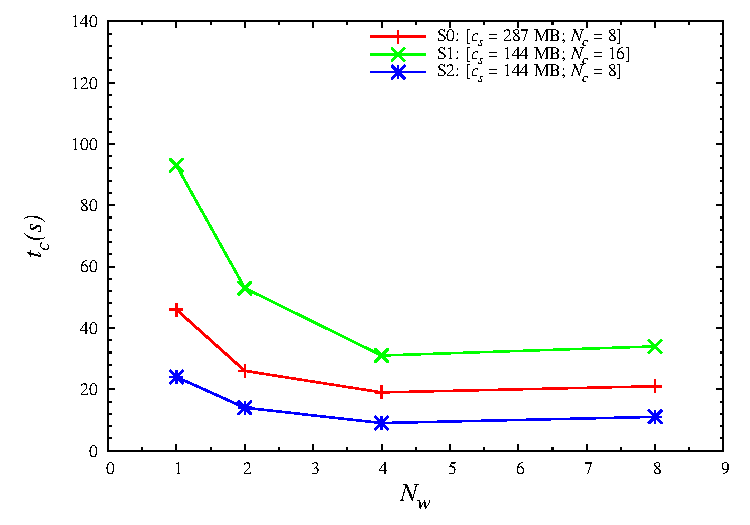
\includegraphics[scale=0.5]{data/graphs/LocalFigure}
\label{Fig:ExpIConventionalLocal:a}
}
\subfigure[$(c_s, N_c, fs, m)=(\mbox{287 MB, 8, local, gridFTP})$]{
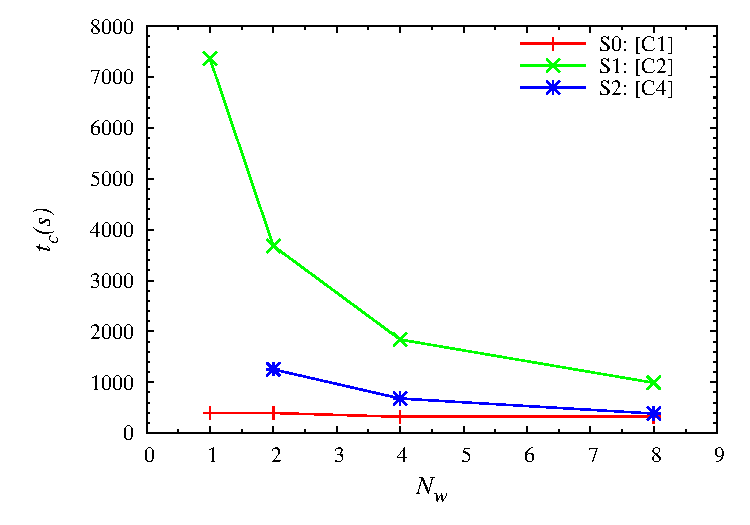
\includegraphics[scale=0.5]{data/graphs/ConventionalFigure}
\label{Fig:ExpIConventionalLocal:b}
}
\caption{\textit{Performance results for All-Pairs using GridFTP for
file reads being compared to a completely local run. Note the scale.}}
\label{Fig:ExpIConventionalLocal}
\end{figure}
\end{center}

\vspace{-0.2in}
In order to properly evaluate all properties of a data-intensive
application in practical use, we added to our last experiment the actual genome
compare computation. The complexity added that is necessary to capture to is
the scaling of computation time when multiple computational resources are
collocated.

%Bety's graph goes here
\jhanote{We need data for compute (comparison) and I/O (only) for
different data-set sizes} \micnote{We need data for three and four
machines (just one graph going from 1 machine to four machines}

%Staging experiment
\subsection{Experiment II: Intelligence Based System}
The second experiment is similar to the first, except the All-Pairs
application observes the data's location before determining whether or
not to assign a certain set of data-dependent computation to an idle
job. Inspired by earlier work~\citep{netperf}, this version of the
application performs an extra step during application startup that
approximates the performance of the network by pinging the hosts that
may be be either a computational resource or a data store. This
information is then assembled into a graph data structure. This graph
is utilised at runtime when the application needs to map an idle worker
to an unprocessed set of pairs defined in the XML file. This changes the
first-available computational resource assignment mechanism described in
the first experiment to an intelligent based system. Though ping is not
very sophisticated in terms of describing a network's behavior, it is a
first-approximation to performance model aware data-placement strategy.
We also experimented with throughput via netperf \citep{netperf_web} as
a method to describe a network's behavior, but since we were working
with such a static set of resources (LONI), the same data graph was
generated as with ping. The netperf-based intelligent system took
approximately 8 seconds longer per resource to run due to the nature of
the network evaluation, but yielded no benefit. These approaches know
where the files are located and their distance to available
computational resources, thus allowing more intelligent decisions when
mapping a set of pairs to a computational resource. An even more
involved approach would be to manage locations of files dynamically at
run-time depending on usage patterns. We leave this approach to future
research.

%Figure 2
\begin{center}
\begin{figure}
\subfigure[*Remove this figure* $(c_s, N_c, fs, m)=(\mbox{287 MB, 8, local, gridFTP})$]
{
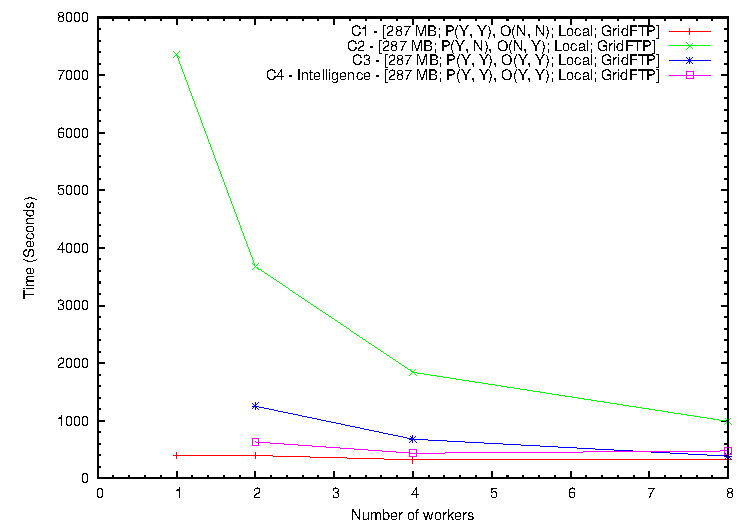
\includegraphics[scale=0.5]
  {data/graphs/IntelligentVsConventionalFigure}
  \label{Fig:IntelligentExp:a}
  }  
\subfigure[$(c_s, N_c, fs, m)=(\mbox{287 MB, 8, local, gridFTP})$]
{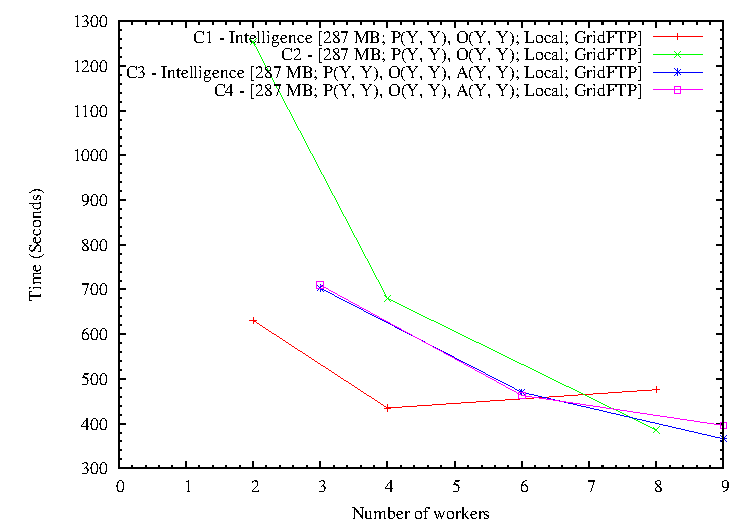
\includegraphics[scale=0.5]
  {data/graphs/IntelligentFigure}
    \label{Fig:IntelligentExp:b}}
\caption{\textit{The figure on the left demonstrations improved
performance with minimal network awareness while the figure, while the
figure on the right demonstrates less performance improvement when more
resources are involved.}}
\label{Fig:IntelligentExp}
\end{figure}
\end{center}

The overhead of intelligence includes the time spent pinging hosts and
building the graph data structure. The total time spent for this
overhead was negligible at approximately two seconds per application
run. In figure \ref{Fig:IntelligentExp:a}, we achieved a great reduction
in time to completion due to the use of intelligence.  However, when the
same tests were performed utilising 3 resources instead of 2, the
intelligence seemed to offer no significant reduction. The explanation
that we propose for this, is that the sets of pairs defined in the XML
file at application start, were geographically dispersed throughout the
network.  Essentially, each set of pairs had approximately the same cost
calculated by using the graph data structure. Each set of pairs would
take the same time to compute using any computational resource.
\jhanote{Perhaps define a test to verify this, so a note can go in
saying we investigated this}

\subsection{Experiment III: CloudStore} 
The third experiment provides information into CloudStore's performance
in handling data locality issues. The same All-Pairs application as in
Experiments 1 and 2 is used, except all data is stored on the
distributed filesystem CloudStore under various configurations. Some
variables of importance include number of data servers that store data,
replication value for data in these data servers, and as above,
placement and number of computational resources.  All read and writes
also utilise the distributed filesystem. Again, for out first set of
results, we focus on $t_{compute}=0$.  
%Figure 3
\begin{center}
\begin{figure}
\subfigure[$(c_s, N_c, fs, m) = (\mbox{287 MB, 8, CloudStore, Direct})$]
{
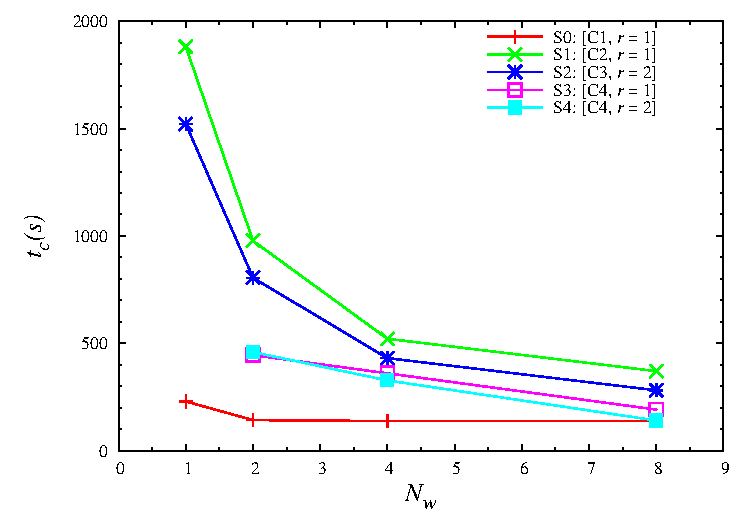
\includegraphics[scale=0.5]  {data/graphs/CloudStoreFigure}
\label{Fig:experiment3:a}
}
\subfigure[$(c_s, N_c, fs, m) = (\mbox{287 MB, 8, CloudStore, Direct})$]
{
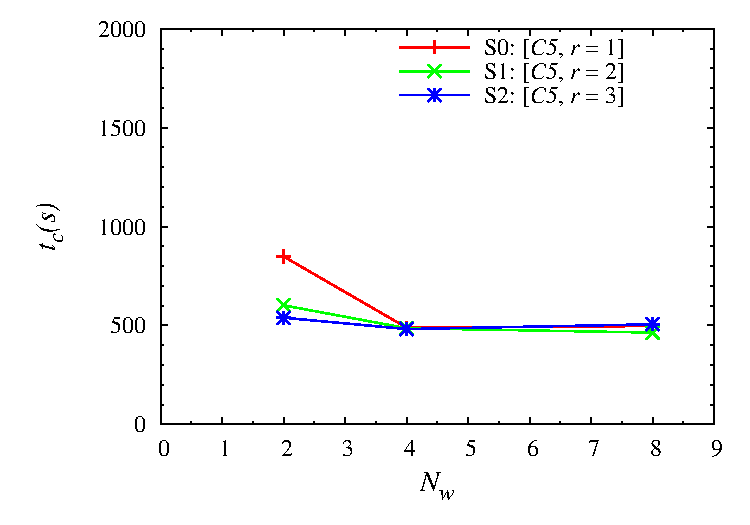
\includegraphics[scale=0.5] {data/graphs/CloudStore3Mach}
\label{Fig:experiment3:b}
}
\caption{\textit{The figure on the left demonstrates All-Pairs'
performance with CloudStore locally and on two different machines. The
other figure demonstrates how this scales to three machines.}
\jhanote{This caption needs attention}}
\label{Fig:experiment3}
\end{figure}
\end{center}

As done above for the first experiment, we have attempted to capture how
compute time scales under these configurations. \micnote{Sentence about
c2 and c3: On the left hand side of figure \ref{Fig:experiment3}, line
C2 has data distant from the computation. Line C3 has data mixed with
some resources. They follow the same curves with line C3 having speed
improvements.} 
%Figure 4
\begin{center}
\begin{figure}
\subfigure[$t_{compute} \ne 0$]
{
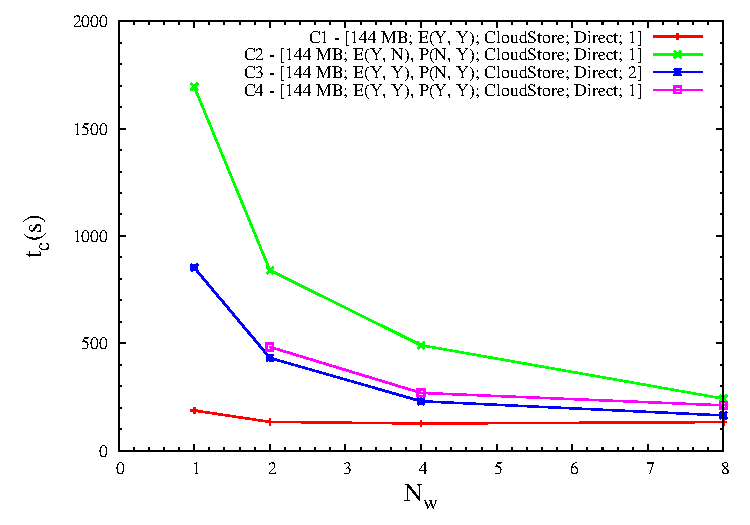
\includegraphics[scale=.5]{data/graphs/CloudStoreCompute}
\label{Fig:experiment4:a}
}
\subfigure[$t_{compute} = 0$]
{
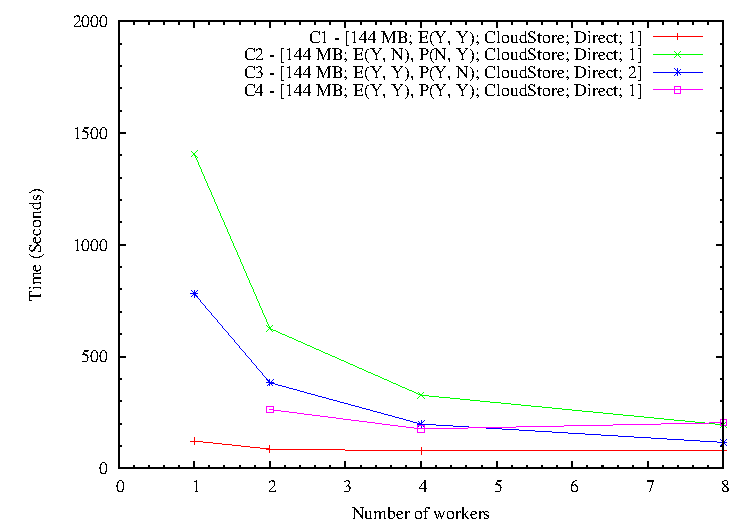
\includegraphics[scale=0.5]{data/graphs/CloudStoreNoComputeSmallerDataSet}
\label{Fig:experiment4:b}
}
\subfigure[Fig. \ref{Fig:experiment4:a} - Fig. \ref{Fig:experiment4:b}, i.e., $\Delta t_c$, $(c_s, N_c, fs, m) = (\mbox{144 MB, 8, CloudStore, Direct})$]
{
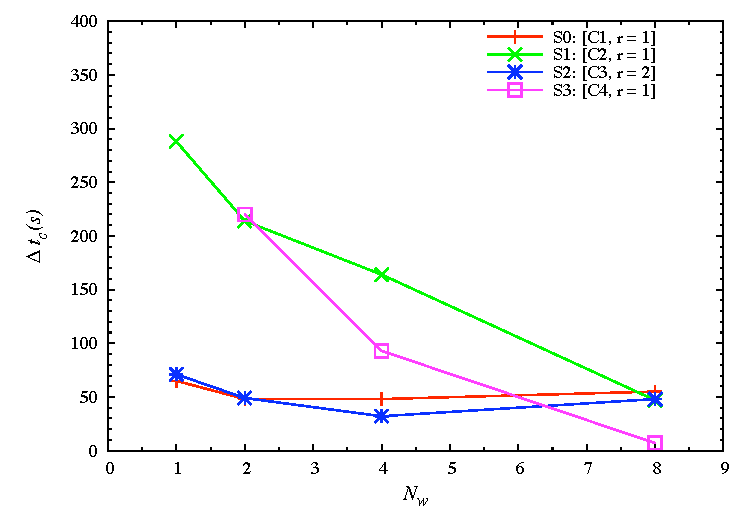
\includegraphics[scale=0.5]{data/graphs/CloudStoreComputeMinusNoCompute144}
\label{Fig:experiment4:c}
}
\caption{\textit{Comparison of CloudStore using the All-Pairs
    application with and without actual computation.} \jhanote{the
    labels need to be fixed, i.e. remove long descriptions}}
\label{Fig:experiment4}
\end{figure}
\end{center}


\begin{center}
\begin{figure}
\subfigure[$\Delta t_c$]
{
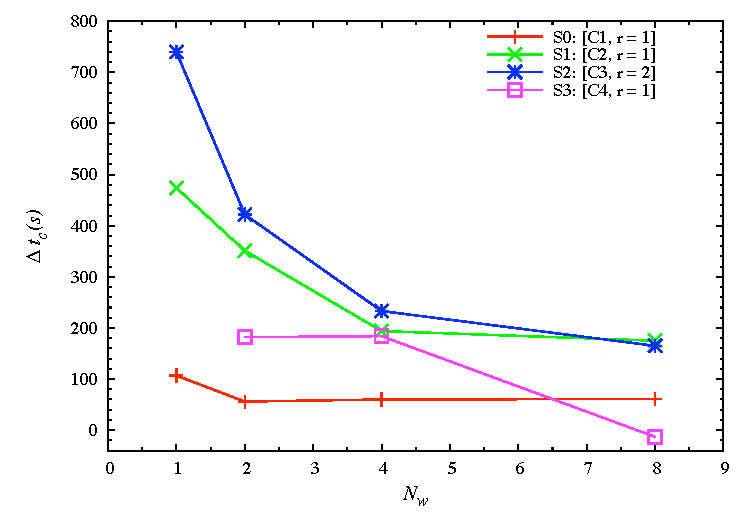
\includegraphics[scale=0.5]{data/graphs/CloudStoreNoCompute_287Minus144}
\label{Fig:CloudStore287minus144:a}
}
\subfigure[$\Delta t_c * N_w$]
{
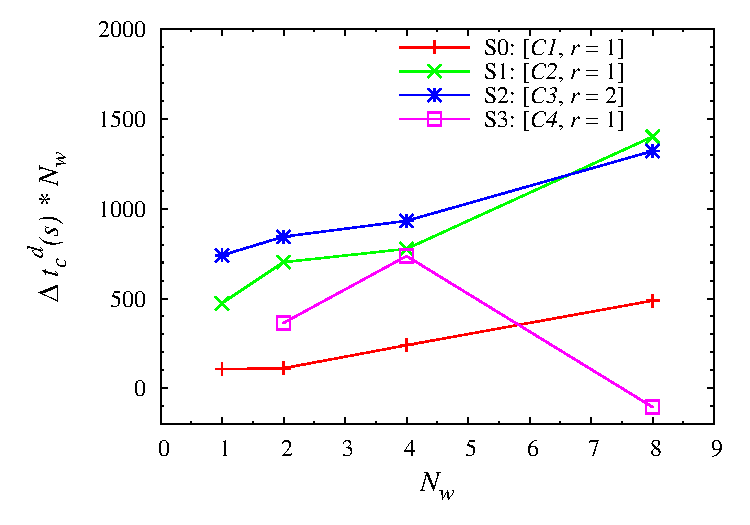
\includegraphics[scale=0.5]{data/graphs/CloudStoreNoCompute_287Minus144TimesNw}
\label{Fig:CloudStore287minus144:b}
}
\subfigure[$t_{common}=2*t(144)-t(287)$]
{
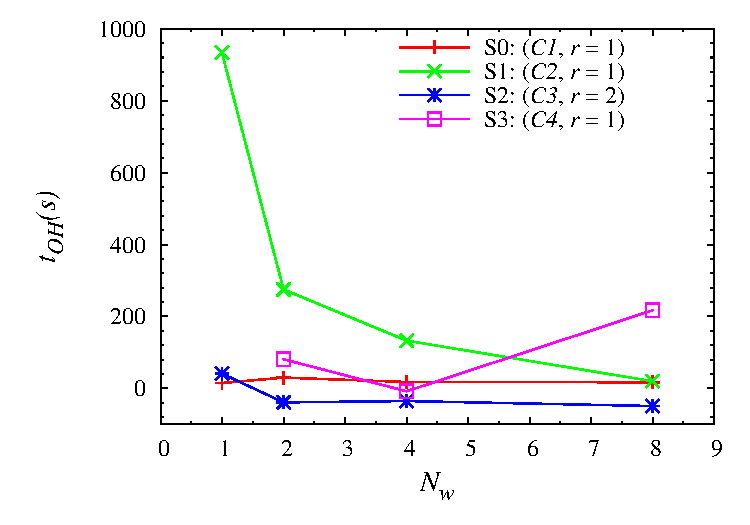
\includegraphics[scale=0.5]{data/graphs/CloudStoreNoCompute_287Minus144CommonTime}
\label{Fig:CloudStore287minus144:c}
}
%%\subfigure[$t_{common}=(2*t(144)-t(287))$*N_w]
%%{
%%\includegraphics[scale=0.5]{data/graphs/CloudStoreNoCompute_287Minus144CommonTimeTimesNw}
%%\label{Fig:CloudStore287minus144:d}
%%}
\caption{\textit{Fig. \ref{Fig:experiment3:a} - Fig. \ref{Fig:experiment4:b}, i.e., $\Delta t_c = t_c(c_s=287 MB, t_{compute}=0) - t_c(c_s=144 MB, t_{compute}=0)$, $(N_c, fs, m) = (\mbox{8, CloudStore, Direct})$}}
\label{Fig:CloudStore287minus144}
\end{figure}
\end{center}

\begin{center}
\begin{figure}
\subfigure[$(c_s, N_c) = (\mbox{287 MB, 8})$]
{
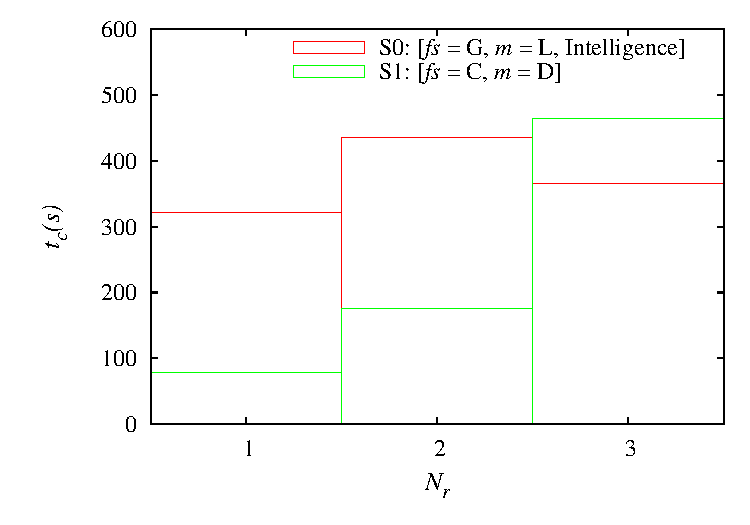
\includegraphics[scale=0.5]{data/graphs/NumberResourcesFigure}
\label{Fig:CloudStoreVsGridFTP:a}
}
\subfigure[$(c_s, N_c, M_c) = (\mbox{287 MB, 8, C5})$]
{
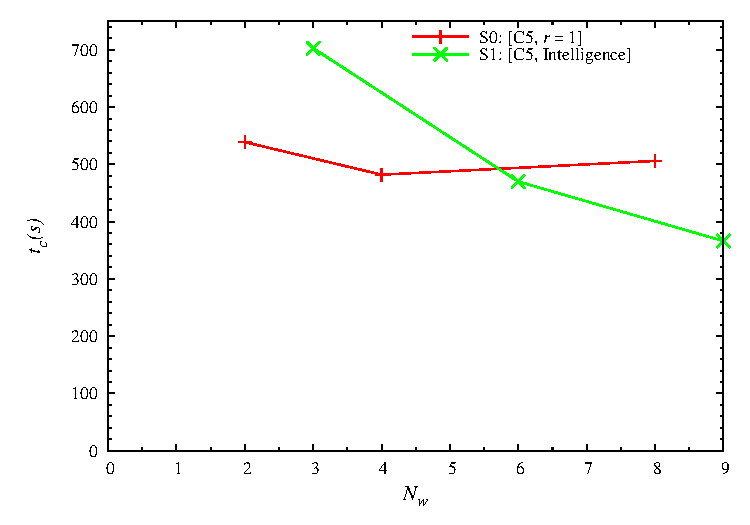
\includegraphics[scale=0.5]{data/graphs/CloudStoreVsGridFTPFigure}
\label{Fig:CloudStoreVsGridFTP:b}
}
\caption{\textit{The figure on the left shows optimal times we achieved
for a given number of resources $(N_{r})$. The figure on the right
demonstrates performance with 3 resources for both GridFTP and
CloudStore.}}
\label{Fig:CloudStoreVsGridFTP}
\end{figure}
\end{center}

%\section{Analysis}

Overall, the use of CloudStore decreases the time to completion
($t_c$) compared to the intelligent and the local approaches. Our
simple intelligent approach did not performed as well as CloudStore, but
works better than the local tests. For the parameters we used, the
introduction of more workers, up to 8 in our case, decreases the time of
completion; however, for the case of a single machine performing as both
master and workers, we hit an I/O bound, probably caused by the network.
For all of our approaches, GridFTP, Intelligent, and CloudStore, we find
the time to completion for three cases: a single machine is the master
and the workers, one machine does the computing while another has the
data stored, and the case when we spread the data into both machines,
while both of them compute.  In all of our three approaches, the case of
a single machine, shows the least $t_c$. In the case of two machines,
having the data in one, and computing in the other one, increases the
time to completion. By splitting the data in both of the machines, and
computing in both, we decrease $t_c$. We then added another case, all
the data in each of machines, and computing in both. This decreases the
time even further, but not to the point of the local computations;
perhaps, all the approaches are not guaranteed to use the data in the
machine the job is being run, even thought the data is in both machines.

???For our three cases,  $t_c$ may be bounded, and decrease to $t_c$(single machine) as  the number of workers ($N_w$) increases, up to a critical $N_w$, after which $T_c$ will increase due to worker coordination overhead.





\section{Analysis}

Overall, the use of CloudStore decreases the time to completion
($t_c$) compared to the intelligent and the local approaches. Our
simple intelligent approach did not performed as well as CloudStore, but
works better than the local tests. For the parameters we used, the
introduction of more workers, up to 8 in our case, decreases the time of
completion; however, for the case of a single machine performing as both
master and workers, we hit an I/O bound, probably caused by the network.
For all of our approaches, GridFTP, Intelligent, and CloudStore, we find
the time to completion for three cases: a single machine is the master
and the workers, one machine does the computing while another has the
data stored, and the case when we spread the data into both machines,
while both of them compute.  In all of our three approaches, the case of
a single machine, shows the least $t_c$. In the case of two machines,
having the data in one, and computing in the other one, increases the
time to completion. By splitting the data in both of the machines, and
computing in both, we decrease $t_c$. We then added another case, all
the data in each of machines, and computing in both. This decreases the
time even further, but not to the point of the local computations;
perhaps, all the approaches are not guaranteed to use the data in the
machine the job is being run, even thought the data is in both machines.

???For our three cases,  $t_c$ may be bounded, and decrease to $t_c$(single machine) as  the number of workers ($N_w$) increases, up to a critical $N_w$, after which $T_c$ will increase due to worker coordination overhead.




\section{Conclusion} Our results show that a DFS greatly changes the
performance of a distributed application in a positive manner. Our
experiments that utilised the DFS to access and store data outperformed
their gridFTP counterparts by an order of magnitude in most cases. Our
results also indicate that the DFS scales better as file sizes and
number of files grow, although both seem to scale linearly. Before any
conclusions may be drawn, there are issues that need to be addressed.
Our application utilised SAGA to access DFS based and gridFTP based
files. Although there is clearly a SAGA induced overhead, this overhead
is constant. \jhanote{ We need to discuss performance issue: Ole has
performance numbers that contradict this, i.e., the overhead that SAGA
introduces for file/gridFTP is very small compared to native globus
calls. This may be due to SAGA's adaptive nature, where lots of
computation is spent determining how to make a distributed call. Other
reason's may be the gridFTP SAGA adaptor being separated from the
application, being able to make only general decisions, allowing no
performance tweaks. Accessing files through this abstraction
with gridFTP seemed to perform sub-optimally in comparison to using the
globus tools directly.} In addition, we were unable to utilise our
entire distributed system, using at most 8 jobs to handle our work.
With a replication level of two in the DFS, data was almost certainly
co-located with the computational resource. In the second experiment,
utilizing information from first staging the network did improve upon
the results of the naive first experiment, but still did not approach
the DFS's performance levels.

Distributed filesystems are important abstractions for a data-intensive
distributed application developers to consider. It also appears that
staging is worth the time required to build a graph representing the
network. Also to note, the second experiment is also naive in the way
that it attempts to optimise data and work assignments. Our staging
only performed pings, not data transfer trials or reliability tests. A
job could have low latency, but poor bandwidth. Perhaps CloudStore's
performance can be attributed to recent work that has shown that data in
large scale distributed applications tends to be accessed together,
despite being seemingly unrelated in the input data-set. Such
correlation in data-access has been observed elsewhere, and specific
abstractions to support the access of ``aggregation of such files'' has
been referred to as a filecule, an application specific group of
files~\citep{filecule}. Attempting to determine if analogous
abstractions could enhance performance for the All-Pair application
could be interesting. In a DFS, however, if the data store is also
capable of data processing, then the DFS is placing commonly used files
together on machines needing them for work; in essence, the DFS is
finding these groups for the developer. The fault tolerance, for which
distributed filesystems are already well renowned for, also has added
benefits to grid application developers in terms of performance. The
distributed application does not have to be aware of where data has been
copied to previously when assigning work; the distributed filesystem
uses the best replica when data is being accessed.

{\bf Acknowledgment:} Important funding for SAGA has been provided by
the UK EPSRC grant number GR/D0766171/1 (via OMII-UK) and HPCOPS
NSF-OCI 0710874. SJ acknowledges the e-Science Institute, Edinburgh
for supporting the research theme, ``Distributed Programming
Abstractions'' and theme members for shaping many important
ideas. This work has also been made possible thanks to the internal
resources of the Center for Computation \& Technology at Louisiana
State University and computer resources provided by LONI. 

%\bibliographystyle{IEEEtran}
\bibliographystyle{kluwer} 
\bibliography{data_intensive_paper}
\end{document}
